% 固定来源 PDF 印刷页 76 第 21 题空间图形的投影示意。
% 空间投影仅表示包含关系与平行/垂直结构，不作为比例图。
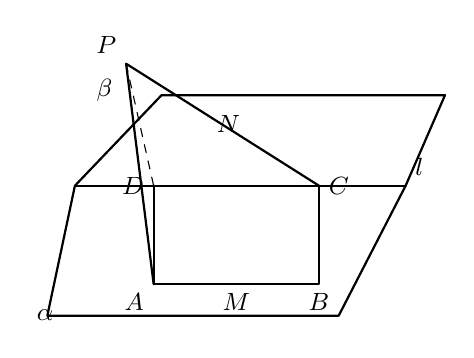
\begin{tikzpicture}[x=1cm,y=1cm,font=\small,line cap=round,line join=round]
  \coordinate (L) at (-.1,0); \coordinate (R) at (4.1,0);
  \coordinate (A1) at (.9,-1.25); \coordinate (B1) at (3.0,-1.25);
  \coordinate (D1) at (.9,0); \coordinate (C1) at (3.0,0);
  \coordinate (P) at (.55,1.55);
  \draw[thick] (L)--(R);
  \draw[thick] (L)--(1.0,1.15)--(4.6,1.15)--(R);
  \draw[thick] (L)--(-.45,-1.65)--(3.25,-1.65)--(R);
  \draw[thick] (A1)--(B1)--(C1)--(D1)--cycle;
  \draw[thick] (P)--(A1) (P)--(C1);
  \draw[dashed] (P)--(D1);
  \draw[thick] (A1)--(D1);
  \node[above left] at (P) {$P$}; \node[below left] at (A1) {$A$};
  \node[below] at (B1) {$B$}; \node[right] at (C1) {$C$}; \node[left] at (D1) {$D$};
  \node[below] at (1.95,-1.25) {$M$}; \node[above] at (1.85,.55) {$N$};
  \node[above right] at (R) {$l$}; \node[above left] at (.5,.95) {$\beta$};
  \node[below left] at (-.25,-1.45) {$\alpha$};
\end{tikzpicture}
